\documentclass[%
 reprint,
%superscriptaddress,
%groupedaddress,
%unsortedaddress,
%runinaddress,
%frontmatterverbose, 
%preprint,
%preprintnumbers,
%nofootinbib,
%nobibnotes,
%bibnotes,
 amsmath,amssymb,
 aps,
%pra,
%prb,
%rmp,
%prstab,
%prstper,
%floatfix,
]{revtex4-2}

\usepackage{graphicx}% Include figure files
\usepackage{dcolumn}% Align table columns on decimal point
\usepackage{bm}% bold math
\usepackage{physics}
\usepackage{cancel}
\usepackage{float}
\usepackage{blindtext}
\usepackage{listings}
\usepackage{titlesec}
% \titlespacing*{\section}{0pt}{0.5\baselineskip}{0.5\baselineskip}
\titlespacing*{\subsection}{0pt}{0.5\baselineskip}{0.5\baselineskip}
%\usepackage{hyperref}% add hypertext capabilities
%\usepackage[mathlines]{lineno}% Enable numbering of text and display math
%\linenumbers\relax % Commence numbering lines

%\usepackage[showframe,%Uncomment any one of the following lines to test 
%%scale=0.7, marginratio={1:1, 2:3}, ignoreall,% default settings
%%text={7in,10in},centering,
%%margin=1.5in,
%%total={6.5in,8.75in}, top=1.2in, left=0.9in, includefoot,
%%height=10in,a5paper,hmargin={3cm,0.8in},
%]{geometry}

\begin{document}

\preprint{APS/123-QED}

\title{Survey of Computational Methods for Plasmas}% Force line breaks with \\

\author{Evan Bluhm}
%  \altaffiliation[Also at ]{Physics Department, XYZ University.}%Lines break automatically or can be forced with \\
% \author{Second Author}%
%  \email{Second.Author@institution.edu}
% \affiliation{%
%  Authors' institution and/or address\\
%  This line break forced with \textbackslash\textbackslash
% }%


\date{June 04, 2021}% It is always \today, today,
             %  but any date may be explicitly specified
\begin{abstract}

Computational models hold an important position in the study of plasma dynamics, complementing the results of analytical models and experimental data. We present example implementations of two of the most commonplace computational methods, a particle-in-cell code and a magnetohydrodynamic code. Each model was applied to a set of standard benchmark problems to validate the accuracy and stability of the numerical models.
% % \begin{description}
% % \item[Usage]
% % Secondary publications and information retrieval purposes.
% % \item[Structure]
% % You may use the \texttt{description} environment to structure your abstract;
% % use the optional argument of the \verb+\item+ command to give the category of each item. 
% % \end{description}
\end{abstract}

%\keywords{Suggested keywords}%Use showkeys class option if keyword
                              %display desired
\maketitle
%\tableofcontents

% \section{Introduction}
\section{Particle-in-Cell Model}
The particle-in-cell (PIC) model samples the velocity distribution at a set of nonuniform spatial locations to define a number of super-particles, which are then subjected to electromagnetic forces. This type of model accurately captures dynamics at small spatial and temporal scales, but becomes computationally infeasible at large temperatures and spatial scales. We have implemented a 1D2V collisionless, magnetostatic PIC model using Python, following the techniques outlined in chapters 1-7 of Ref. \cite{BirdsallCharlesK1991Ppvc}.
\subsection{Particle Weighting and Field Solver}
In the PIC method, we treat particles as having a finite extent, rather than point particles. The forces acting on the particles are those of the long-range electromagnetic fields, which we compute at a finite set of points on a uniform grid. This method resolves the issue of treating $N$ singularities in the Coulomb force, and absolves us of the need to compute $N^2$ particle-particle interactions. Particles are weighted to the grid according to the assumed shape profile, giving the source terms for the Maxwell equations. Once fields on the grid have been computed, the force on each particle is assigned in turn by a similar weighting process. The weighting process for zeroth-order and first-order weighting is described in chapter 2 of Ref. \cite{BirdsallCharlesK1991Ppvc}.

At each time step, we solve for the forces on all particles by estimating the electric field at each particle's location. In the magnetostatic model the magnetic field is constant, so we may solve Poisson's equation for the electric scalar potential $\phi$, and calculate its gradient:
\begin{eqnarray}
\nabla ^2 \phi & = & - \rho_c / \epsilon_0 \\
\vec E & = & - \grad \phi
\end{eqnarray}
where $\rho_c$ is the charge density. Weighting the particles to the grid gives $\rho_j$. For meaningful results, the overall charge density of the system must be zero, so a constant background of opposite charge is added to $\rho_j$ to enforce charge neutrality. We also absorb the $\epsilon_0$ normalization into $\rho_j$. The finite difference method used to solve Poisson's equation is detailed in Appendix B.
\subsection{Integrator}
The PIC method uses a leap-frog integration scheme, with particle position and velocity are separated in time by ($\Delta t/2$), so that the average value of $\vec x$ over the step is used to calculate $\Delta \vec v$, and vice-versa. If a non-zero magnetic field is provided, a Strang splitting of the particle advance is performed, applying the rotation due to the magnetic field halfway between half-steps of the leapfrog time step. Use of a symplectic integration scheme improves the conservation properties of the model. To start the leapfrog integrator, the model performs a single iteration of a backwards integrator to find $v_i ^{-1/2}$ from the initial conditions.

The spatial boundaries of the PIC model are assumed to be periodic with length $L$, such that $x + L = x$.
\subsection{Normalization}
Quantities have been normalized such that the scales of interest are of order unity. The plasma frequency $\omega_p$, the electric constant $\epsilon_0$, and the charge-to-mass ratio of the particles $q/m$ are inputs to the program, determining the time, mass, and charge scales. The initial positions and velocities of the particles determine the units of length. This normalization results in quantities that are easy to compare and visualize at similar absolute scales, while minimizing floating point errors.
\subsection{Code Structure}
The model implementation was structured within three abstract separate Python classes to allow for a variety of configurations and integration methods. The problem configuration is stored in an instance of the \texttt{Configuration} class, which contains each model parameter that does not change over the course of a simulation. An instance of the \texttt{Configuration} class defines an \texttt{init()} method which sets the initial position and velocity of each particle. Various problem configurations, for example a pair of counter-streaming beams, are easily defined by inheriting the \texttt{Configuration} class, as shown in Appendix A.

A \texttt{ParticleData} structure stores the current state of the ensemble, historical snapshots of the configuration over time, and the history of any desired diagnostics. To maintain reasonable memory consumption over the course of a simulation run, the full state is stored at a subsampled rate. Finally, the \texttt{PicModel} class defines the integration method and boundary conditions for the problem, taking as input a \texttt{Configuration} instance and using a \texttt{ParticleData} instance to store the system state. A \texttt{PicModel} instance may be written directly to hard disk, allowing for both resumption of a previous simulation, as well as easy post-hoc data analysis.
\subsection{PIC Applications}
We applied our PIC model to several benchmark problems with known solutions, in order to validate the accuracy and stability of the model. A pair of stationary particles were shown to oscillate at the plasma frequency, as expected. The leap-frog integration method itself is numerically unstable when $\omega_p \Delta t > 2$. The leap-frog instability was demonstrated by simulating a cold plasma with a small oscillatory perturbation, using increasing values of $\Delta t$.

The two-stream instability is an important unstable system which can be reproduced by a surprisingly low-fidelity PIC model. For a static equilibrium of two cold, counter-streaming beams, small perturbations will grow exponentially in time. Linear analysis of the Vlasov equation gives the dispersion relation:
\begin{equation}
1 - \frac{1}{2} \left( \frac{\omega_p ^2}{(\omega - k v_0)^2} + \frac{\omega_p ^2}{(\omega + k v_0)^2}\right) = 0
\end{equation}
where $\omega_p$ is the usual plasma frequency. The solutions are:
\begin{equation}
\omega = \pm \sqrt{k^2 v_0 ^2 + \omega_p ^2 \pm \omega_p \sqrt{4 k^2 v_0 ^2 + \omega_p ^2}}
\end{equation}
For $k v_0 / \omega_p < \sqrt{2}$, there are imaginary solutions for $\omega$, which will grow exponentially in time as shown in Figure \ref{fig:two-stream-k=1-snapshots}. The exponential growth observed by the PIC model agrees with the growth rate predicted by the linear theory.
\begin{figure}
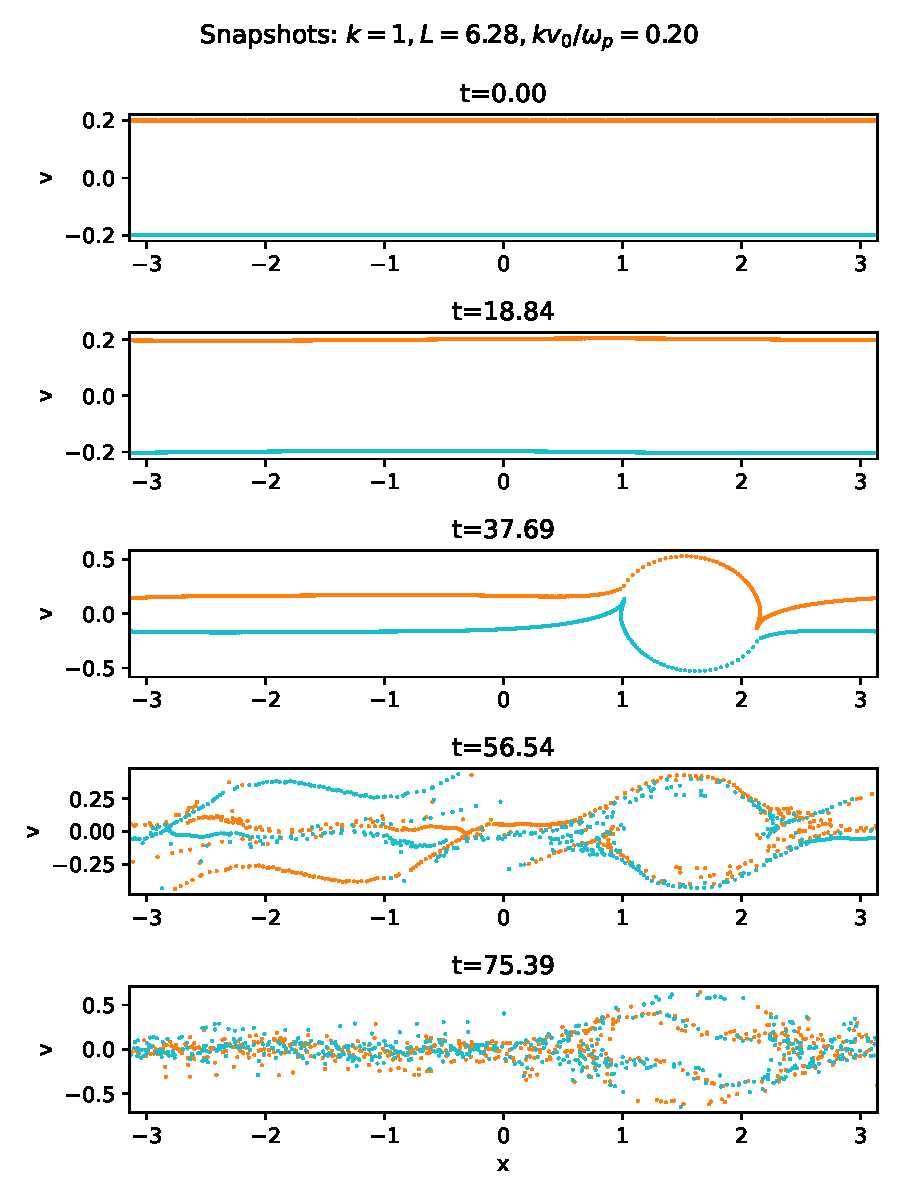
\includegraphics[width=0.9\linewidth]{proj3/two-stream-k=1-snapshots.pdf}
\caption{\label{fig:two-stream-k=1-snapshots}Snapshots of the growth of the $k=1$ two-stream instability over time. Orange particles are initially streaming to the right, and blue particles are initially streaming to the left. $k v_0 / \omega_p = 0.2$, units of time are $1/\omega_p$. The initially small perturbation grows exponentially, appearing as a stationary vortex in phase space. The unstable mode reaches nonlinear saturation after fewer than 10 periods of the plasma frequency. The exponential growth rate of the unstable mode agrees with the rate predicted by the linearized Vlasov equations.}
\end{figure}

The Dory-Guest-Harris instability describes the conditional stability of a magnetized ring distribution \cite{PhysRevLett.14.131}. Unstable modes are possible for certain values of the cyclotron frequency $\omega_c$, the ring velocity $v_\perp$, and the perturbation wavenumber $k$. The solutions to the linearized Vlasov equation for a magnetized cold ring distribution have complex solutions, featuring both oscillations and exponential growth. Our PIC code demonstrates the instability, as shown in Figure \ref{fig:dory-guest-harris-4.10}. A particular wavenumber $k$ was excited by initializing an appropriately periodic velocity perturbation in the initial cold ring distribution. Measuring the growth rate and oscillation frequency of the electric field energy gave good agreement with the values predicted by the dispersion relation.

The growth rates and oscillation frequency of the Dory-Guest-Harris instability were also used to validate the accuracy of the PIC solver. The leap-frog integration scheme used should be second-order accurate. By performing simulations with varying grid sizes and the same model parameters, we observed quadratic convergence of the instability growth rate to the exact solution.
\begin{figure}
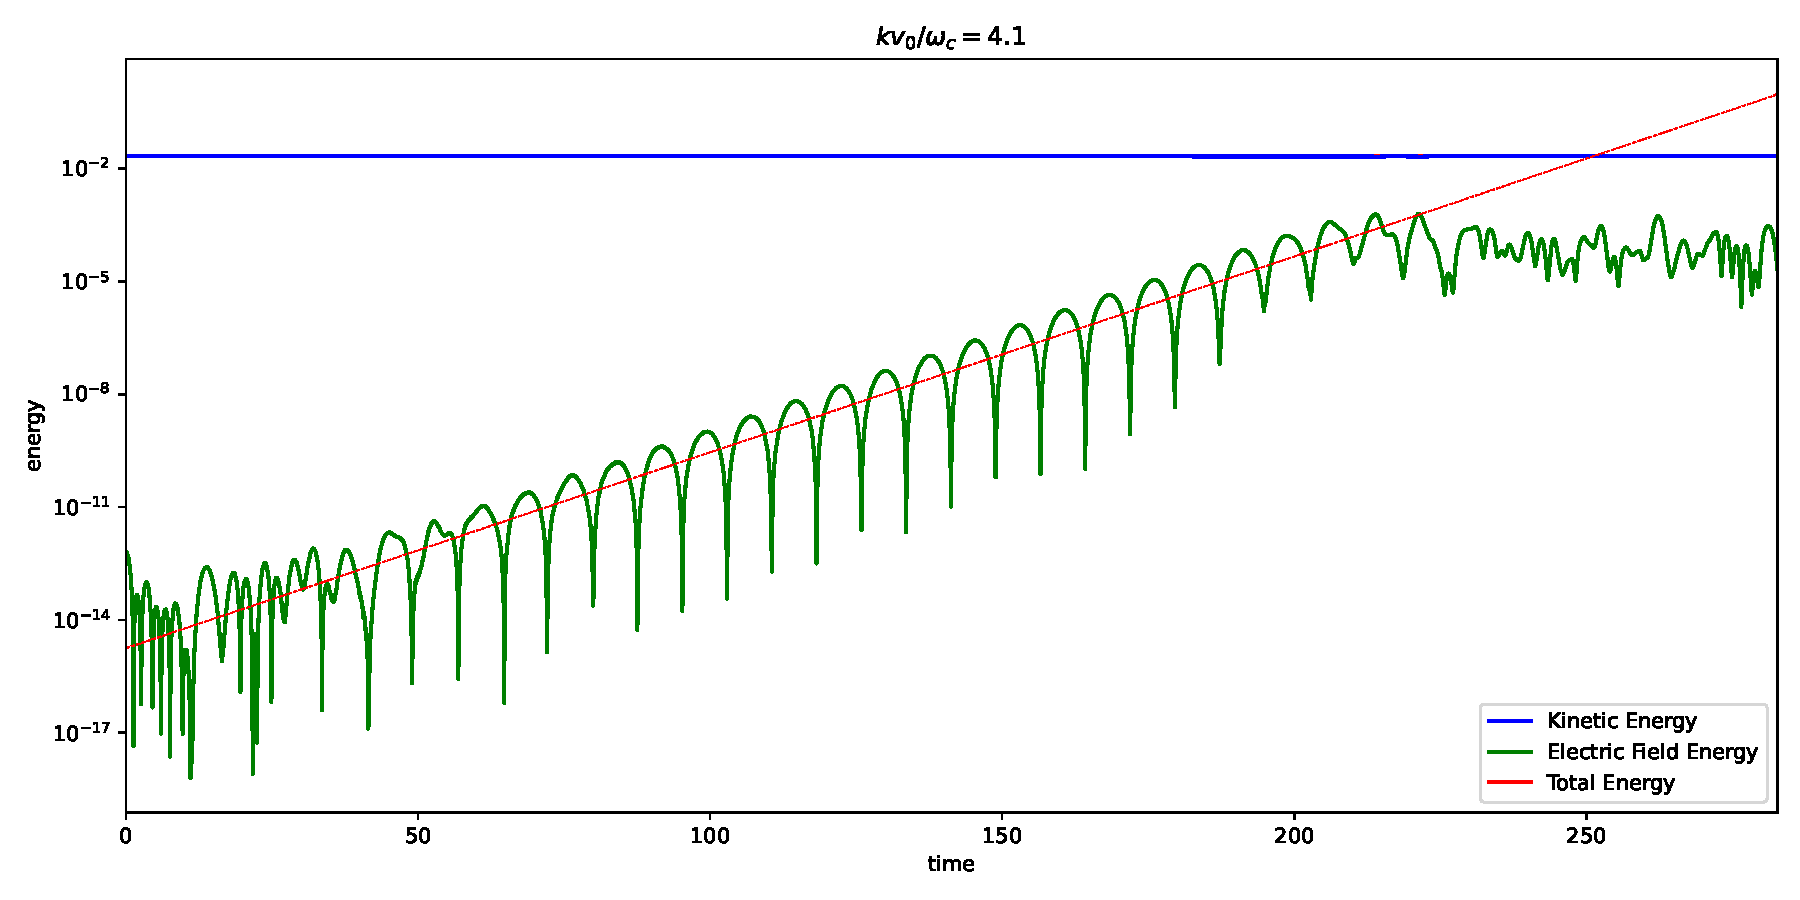
\includegraphics[width=0.9\linewidth]{proj4/dgh_4.10.pdf}
\caption{\label{fig:dory-guest-harris-4.10}Demonstration of the Dory-Guest-Harris instability for a cold ring distribution. Growth and oscillation of the electric field energy over time demonstrates the presence of an excited mode with a complex $\omega$. In this simulation, $\omega_c = 1/\sqrt{10}$, $\omega_p = 1$, $k = 1$ and $v_\perp = 1.42$. Time is normalized by the plasma frequency. The least squares regression fit to the period of linear growth is shown as a red dashed line. The slope of the exponential growth is the complex part of $\omega$, and the oscillation frequency is the real part, giving $\omega / \omega_c = 1.30 + 0.190i$, to good agreement with the analytic dispersion relation.}
\end{figure}
\section{Magnetohydrodynamic Model}

The equations of ideal magnetohydrodynamics (MHD) capture much of the behavior of well-magnetized plasmas which have a high degree of ion collisionality and low resistivity. Using a fluid description allows us to model phenomena at much larger spatial and temporal scales. We implemented a fully 3-dimensional MHD solver using a MacCormack finite difference scheme to integrate the nonlinear ideal MHD equations in conservative form. The solver includes additional artificial viscosity to reduce dispersive errors. The stability and accuracy of the implementation were benchmarked against a standard test of MHD solvers, the Brio-Wu shock tube test. The code structure of our ideal MHD solver mimics the \texttt{Configuration}/\texttt{Model}/\texttt{Data} structure of the PIC implementation.

\subsection{Integrator}

The equations of ideal MHD can be written in conservative form as:
\begin{equation}
\pdv{}{t}\vec Q + \div \vec T = 0 
\end{equation}
\begin{equation}
\vec Q = [\rho, \rho v_x, \rho v_y, \rho v_z, B_x, B_y, B_z, e]
\end{equation}
\begin{equation}
\vec T = \begin{bmatrix}
\rho \vec v \\
\rho \vec v \vec v - \frac{\vec B \vec B}{\mu_0} - \left( p + \frac{B^2}{2 \mu_0} \right) \vec{1} \\
\vec v \vec B - \vec B \vec v \\
\left( e + p + \frac{B^2}{2 \mu_0} \right) \vec v - \frac{\vec B \cdot \vec v}{\mu_0} \vec B \label{eqn:ideal-mhd-conservative}
\end{bmatrix}
\end{equation}
where $\rho$ is the plasma mass density, $\vec v$ is the center-of-mass velocity, $\vec B$ is the local magnetic field, $p$ is the plasma pressure, and $e$ is the energy density:
\begin{equation}
e = \frac{p}{\gamma - 1} + \frac{1}{2} \rho v^2 + \frac{B^2}{2 \mu_0}
\end{equation}
Our code attempts to numerically solve the ideal MHD equations by approximating equation (\ref{eqn:ideal-mhd-conservative}) using the MacCormack method, which is second-order accurate in time and space. Stepping forwards in time is done in two steps. First, a predictor step uses a forward difference to estimate the value of $Q$ at time $t = (n+1)\Delta t$:
\begin{eqnarray*}
\overline{Q} _{i,j,k} ^{n+1} & = & Q_{i,j,k} ^n - \frac{\Delta t}{\Delta x} (F_{i+1, j, k}^n - F_{i, j, k} ^n) \\
& & - \frac{\Delta t}{\Delta y} (G_{i, j+1, k} ^n - G_{i, j, k} ^n) - \frac{\Delta t}{\Delta z} (H_{i, j, k+1} ^n - H_{i, j, k} ^n)
\end{eqnarray*}
where $F$, $G$, and $H$ are the fluxes in the x, y, and z directions:
\begin{equation}
\pdv{Q}{t} + \pdv{F}{x} + \pdv{G}{y} + \pdv{H}{z} = 0
\end{equation}
and $F_{i, j, k} ^n$ is the value of $F$ evaluated using the value of $Q_{i, j, k} ^n$. The corrector step is a backwards difference using the estimated value  $\overline{Q}$:
\begin{eqnarray*}
\overline{\overline{Q}} _{i,j,k} ^{n+1} & = & Q_{i,j,k} ^n - \frac{\Delta t}{\Delta x} (\overline{F}_{i, j, k}^n - \overline{F}_{i-1, j, k} ^n ) \\
& & - \frac{\Delta t}{\Delta y} (\overline{G}_{i, j, k} ^n - \overline{G}_{i, j-1, k} ^n) - \frac{\Delta t}{\Delta z} (\overline{H}_{i, j, k} ^n - \overline{H}_{i, j, k-1} ^n)
\end{eqnarray*}
Finally, we obtain the value of $Q$ at time $t = (n+1) \Delta t$ by averaging $\overline{Q}_{i,j,k}$ with $\overline{\overline{Q}}_{i,j,k}$
\subsection{Artificial Diffusion}

Finite difference approximations to hyperbolic partial differential equations can be prone to large oscillatory errors in the vicinity of steep gradients or discontinuities. The spatial average performed when combining the predictor and corrector steps has a diffusive effect on the solution, helping to smooth out oscillatory errors. In some cases, such as the Brio-Wu shock test described below, this is insufficient to maintain stability, and additional artificial diffusion is required. Our code contains a flag called \texttt{diffusion\_method} which determines whether to add an artificial viscosity term, so that instead we solve the following modified system of equations:
\begin{equation}
\pdv{Q}{t} + \pdv{F}{x} + \pdv{G}{y} + \pdv{H}{z} = \sigma \nabla ^2 Q
\end{equation}
where the viscosity $\sigma$ is a configurable parameter. By default, it is everywhere set to a constant value of $\sigma = 0.1 \frac{\Delta x ^2}{\Delta t}$.

\begin{figure}
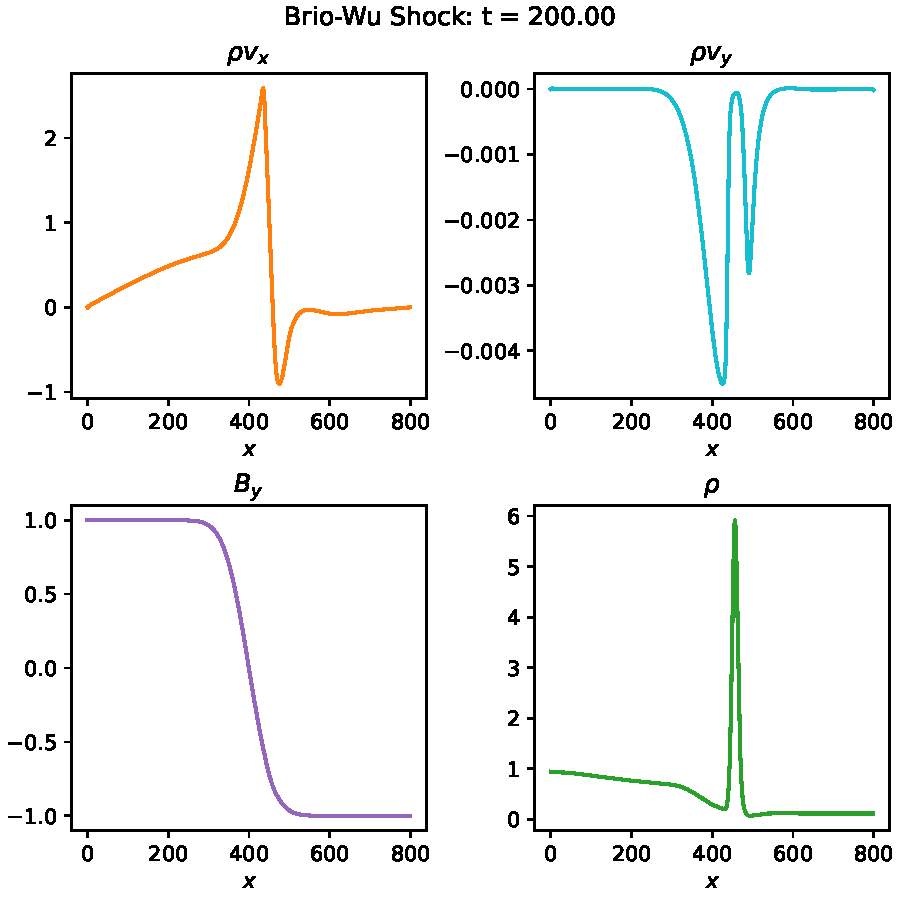
\includegraphics[width=0.7\linewidth]{summary/shock_snapshots_n_20.pdf}
\caption{\label{fig:brio-wu-snapshot}Snapshot of our solver's solution to the standard Brio-Wu shock problem. The solution from our MHD solver is shown after evolving to $t=200$ with artificial viscosity turned on. Non-physical dispersive errors have generated a density spike near $x=440$.}
\end{figure}

\subsection{Stability}

Since the ideal MHD equations are hyperbolic, they support both forward and backward-propagating waves, with characteristics given by the sound speed, the Alfvén speed, and the slow and fast magnetosonic wave speeds. By incorporating both forward and backward differences, the MacCormack scheme is stable to waves propagating in both directions as long as the CFL condition is satisfied for waves with speed $a$:
\begin{equation}
C = \frac{a \Delta t}{\Delta x} < 1
\end{equation}
The fastest-moving wave in ideal MHD is the fast magnetosonic wave. In the x-direction, the fast magnetosonic wave travels at:
\begin{equation}
|v_{fast, x}| = |v_x| + \sqrt{\frac{1}{2}\left(a^2 + c_s ^2 - \sqrt{(a^2 + c_s ^2)^2 - 4 a_x ^2 c_s ^2} \right) }
\end{equation}
where the Alfvén wave speed and sound speed are:
\begin{equation}
a^2 = \frac{B^2}{\rho \mu_0} \qquad a_x ^2 = \frac{B_x ^2}{\rho \mu_0} \qquad c_s ^2 = \frac{\gamma p}{\rho}
\end{equation}
At each time step, our finite difference solver computes the Courant number at each spatial position based on the maximum possible characteristic in each direction. If the CFL stability condition is violated at any point, in any direction, the solver exits with an appropriate message.

\subsection{MHD Applications}

As first shown in Ref. \cite{BRIO1988400}, an extension of the hydrodynamic Sod shock tube to the realm of magnetohydrodynamics is a useful test problem for MHD codes. The Brio-Wu shock tube test is posed as a 1.5D Riemann problem, with a discontinuity in the middle of the domain. Our model's solution for the Brio-Wu shock problem is shown in Figure \ref{fig:brio-wu-snapshot}. The simulation was first performed without artificial diffusion, but Gibbs phenomenon at the discontinuity generated negative densities within a few time steps, and the simulation was terminated early by the physicality checks. The expected forward and backward fast rarefaction waves are easily identifiable in the animated solution, as they are the first to travel away from the discontinuity. However, these waves are not captured in $B_y$. Worse yet, dispersive errors have generated a non-physical spike in the density which grows over time. We were not able to resolve the instability by increasing the artificial viscosity, indicating more fundamental errors in the finite difference solver.

Our ideal MHD solver was also applied to a stationary screw pinch with a parabolic axial current and constant axial magnetic field. The screw pinch equilibrium should be stable in time, but in our model we see the rapid growth of an axisymmetric rotational mode which quickly disrupts the configuration. We conclude that our finite difference approximation to the ideal MHD equations contains outstanding implementation errors.

\subsection{Linearized Ideal MHD Stability Analysis}

In addition to the nonlinear ideal MHD solver, our model also includes a finite difference solver for the linearized ideal MHD equations. The linearized solver uses a forward-time, centered-space difference method to evolve perturbed solutions about a static, axisymmetric equilibrium. The governing equations and finite difference method are detailed in Appendix C. We applied our model to the  axisymmetric force-free spheromak configuration described in Reference \cite{BondesonA1981Tioa} in an attempt to reproduce the well-known $L/R$ stability condition. The symmetry axis proved to be a difficult boundary condition, and numerical instability near $r=0$ dominated the model results, even in stable regimes.

\section{Conclusions}

Particle-in-cell and magnetohydrodynamic single-fluid models only cover a small subset of the rich world of computational models. In the process of implementing both types of model, we can draw some similarities and differences. The relative simplicity of the governing equations for the PIC method made the implementation and debugging process much easier, and allowed for a larger number of simple test configurations, compared with the MHD method. In both cases, correct treatment of the boundaries accounted for a majority of the implementation effort, even for the highly idealized boundary conditions used in our models.

The author has gained a deep respect for the amount of effort and detail required to accurately simulate even the simplest plasma phenomena. Behind the compact form of (\ref{eqn:ideal-mhd-conservative}) hide numerous instabilities and other numerical difficulties which must be carefully considered before a modeler can hope to obtain meaningful, trustworthy results.

\nocite{*}

\bibliography{summary}% Produces the bibliography via BibTeX.

\onecolumngrid

\pagebreak

\appendix

\section{Model Class Inheritance}

To demonstrate the versatility of the inheritance-based \texttt{Configuration} class, the following code listing contains the complete source code required to model two separate problems, including visualizations. The configurations are a warm Gaussian beam, and the perturbed two-stream system shown in Figure \ref{fig:two-stream-k=1-snapshots}.

\begin{lstlisting}[basicstyle=\small]
import numpy as np

from pic1.configuration import Configuration
from pic1.model import PicModel
import pic1.plots as plots

class GaussianBeamConfiguration(Configuration):
    N = 6400  # Number of particles
    M = 512  # Number of grid points
    (x_min, x_max) = (-np.pi, np.pi)  # Spatial domain extent
    wp = 1.0  # Electron plasma frequency
    dt = 0.5  # Time step
    n_periods = 8  # Number of periods of the plasma frequency to simulate

    def set_initial_conditions(self):
        self.initial_x = np.linspace(self.x_min, self.x_max, self.N + 1)[:-1]
        self.initial_vx = np.random.normal(0, 0.1, self.N) + 1
        self.initial_vy = np.zeros_like(self.initial_vx)


c1 = GaussianBeamConfiguration()
m1 = PicModel(c1)
m1.run()
plots.plot_initial_distribution(m1)
plots.animate_phase_space(m1)

class TwoStreamConfiguration(Configuration):
    N = 1024
    M = 512
    wp = 1
    dt = 0.01
    n_periods = 15
    weighting_order = 1
    k = 1
    (x_min, x_max) = (-np.pi / k, np.pi / k)

    def set_initial_conditions(self):
        v0 = 0.2
        delta = 0.001
        beam1_x = (
            np.linspace(self.x_min, self.x_max, int(self.N / 2) + 1)[:-1]
        )
        shift = delta * np.sin(self.k * beam1_x)
        beam1_x += shift
        beam2_x = (
            np.linspace(self.x_min, self.x_max, int(self.N / 2) + 1)[:-1]
        )
        beam1_v = v0 * np.ones_like(beam1_x)
        beam2_v = -v0 * np.ones_like(beam2_x)
        self.initial_x = np.concatenate([beam1_x, beam2_x])
        self.initial_vx = np.concatenate([beam1_v, beam2_v])
        self.initial_vy = np.zeros_like(self.initial_vx)

c2 = TwoStreamConfiguration()
m2 = PicModel(c2)
m2.run()
plots.plot_initial_distribution(m2)
plots.animate_phase_space(m2)
\end{lstlisting}

\section{Solving Poisson's Equation}

In the particle-in-cell model, we must solve Poisson's equation to calculate the electrostatic forces on the grid, using the charge density $\rho_c$ weighted to the grid:
\begin{equation}
\nabla ^2 \phi = - \rho_c / \epsilon_0
\end{equation}

The program uses a finite difference method to solve Poisson's equation for $\phi_j$, and to compute $E_j$. The finite difference operators used are:

\begin{eqnarray}
\frac{\phi^n _{j+1} - 2 \phi_j ^n + \phi^n_{j-1}}{\Delta x ^2} = - \rho _j ^n \\
E_j ^n = - \frac{\phi ^n _{j+1} - \phi ^n _{j-1}}{2 \Delta x}
\end{eqnarray}

Poisson's equation in this finite difference form can be expressed as a matrix equation $\vec A \vec \phi = \vec \rho $. Solving for $\vec \phi$ is as simple as inverting $\vec A$. For our system with periodic boundary conditions, however, the solution $\vec \phi$ is lacking a gauge and, with the result that $\vec A$ is singular. In the program, we resolve the gauge ambiguity by setting $\phi_0 = 0$, and disregard the value of $\rho_0$ as it is redundant. We can write the resulting matrix equation in the following form:

\begin{equation}
\frac{1}{\Delta x ^2}\begin{bmatrix}
1 & 0 & 0 & 0 & \ldots & 0 \\
1 & -2 & 1 & 0 & \ldots & 0 \\
0 & 1 & -2 & 1 & \ldots & 0 \\
 & \ldots & \ldots & \ldots &  & 0 \\
0 & \ldots & 1 & -2 & 1 & 0 \\
0 & \ldots & 0 & 1 & -2 & 1 \\
-1 & \ldots & 0 & 0 & 1 & -2 \\
\end{bmatrix} \begin{bmatrix}
\phi_0 \\ \phi_1 \\ \phi_2 \\ \phi_j \\ \phi_{m-3} \\ \phi_{m-2} \\ \phi_{m-1} 
\end{bmatrix} = \begin{bmatrix}
0 \\ \rho_1 \\ \rho_2 \\ \rho_j \\ \rho_{m-3} \\ \rho_{m-2} \\ \rho_{m-1} 
\end{bmatrix}
\end{equation}

With the symmetry broken, this matrix is invertible. The inverted $\vec A^{-1}$ is constant throughout the time integration, and is only computed once at the beginning of the run. The functions to compute both $\vec A^{-1}$ and $E_j$ are included in the \texttt{poisson.py} module. A set of associated \texttt{pytest} test cases use constructed solutions to validate that the finite difference method is accurate to the expected $O(\Delta x ^2)$.


\section{Finite Difference Solution of Time-Dependent Linear MHD Equations}

For a static equilibrium $\rho_0, \vec v _0, \vec B_0, p_0$ with a small perturbation $\rho_1(t), \vec v_1(t), \vec B_1(t), p_1(t)$, we discard terms which are second-order in perturbation quantities. The resulting linearized ideal MHD equations for a static equilibrium ($\vec v_0 = 0$) are:

\begin{equation}
\pdv{\rho_1}{t} = - \div ( \rho_0 \vec v_1)    
\end{equation}
\begin{equation}
\pdv{p_1}{t} = - \div (p_0 \vec v _1) + (1 - \gamma) p_0 \div \vec v_1 
\end{equation}
\begin{equation}
\pdv{\vec B_1}{t} = \curl ( \vec v_1 \cross \vec B_0)
\end{equation}
\begin{equation}
\rho_0 \pdv{\vec v_1}{t} = \grad p_1 + \frac{1}{\mu_0} \left[ (\curl \vec B_1) \cross \vec B_0 + (\curl \vec B_0) \cross \vec B_1 \right]
\end{equation}

For a cylindrical equilibrium, we assume angular dependence of the perturbation is:
\begin{equation}
g_1 (r, \theta, z, t) = g_1(r, z, t) e^{i m \theta}
\end{equation}
\begin{equation}
\text{Re}(g_1) = g_1(r, \theta=0, z, t)
\end{equation}
\begin{equation}
\text{Im}(g_1) = g_1(r, \theta=- m \pi/2, z, t)
\end{equation}
such that
\begin{equation}
\pdv{g_1}{\theta} = i m g_1
\end{equation}

For the purposes of our model, we will also limit ourselves to equilibria with:
\begin{equation}
\grad p_0 = 0
\end{equation}
\begin{equation}
\grad \rho_0 = 0
\end{equation}
\begin{equation}
\pdv{\vec B_0}{\theta} = 0
\end{equation}

To make the notation a bit easier to read, let
\begin{equation}
\vec B_0 = B_r \vu r + B_\theta \vu \theta + B_z \vu z
\end{equation}
\begin{equation}
\vec B_1 = b_r \vu r + b_\theta \vu \theta + b_z \vu z
\end{equation}
\begin{equation}
\vec v_1 = u \vu r + v \vu \theta + w \vu z
\end{equation}

With these assumptions, we can write the linearized ideal MHD equations for a cylindrical equilibrium with complex-valued $\vec b$ and $\vec v_1$ as:

\begin{equation}
\pdv{\rho_1}{t} = - \left( \frac{1}{r} \pdv{( r \rho_0 u)}{r} + \frac{1}{r} \pdv{(\rho_0 v)}{\theta} + \pdv{(\rho_0 w)}{z} \right)
\end{equation}
\begin{equation}
\pdv{p_1}{t} = - \gamma p_0 \left( \frac{1}{r} \pdv{(r u)}{r} + \frac{1}{r} \pdv{v}{\theta}  + \pdv{w}{z}  \right)
\end{equation}
\begin{equation}
\pdv{b_r}{t} = - w \pdv{B_r}{z} + \frac{1}{r} \left[ r B_z \pdv{u}{z} + r u \pdv{B_z}{z} + i m u B_\theta - B_r (r \pdv{w}{z} + i m v) \right]
\end{equation}
\begin{equation}
\pdv{b_\theta}{t} = - w \pdv{B_\theta}{z} + i m B_z v + v \left( \pdv{B_z}{z} + \pdv{B_r}{r} \right) - u \pdv{B_\theta}{r} - B_\theta \left( \pdv{w}{z} + \pdv{u}{r} \right) + B_r \pdv{u}{r}
\end{equation}
\begin{equation}
\pdv{b_z}{t} = \frac{1}{r} \left[ B_\theta \pdv{w}{\theta} + w \left(B_r + r \pdv{B_r}{r} \right) - r u \pdv{B_z}{r} - B_z \left(u + imv + r \pdv{u}{r} \right) + r B_\theta \pdv{w}{r} \right]
\end{equation}
\begin{equation}
\rho_0 \pdv{u}{t} = \pdv{p_1}{r} + \frac{1}{r \mu_0} \left[ r b_z \left( \pdv{B_r}{z} - \pdv{B_z}{r} \right) - r b_\theta \pdv{B_\theta}{r} + r B_z \left( \pdv{b_r}{z} - \pdv{b_z}{r} \right) + B_\theta \left( -2 b_\theta + i m b_r - r \pdv{b_\theta}{r} \right) \right]
\end{equation}
\begin{equation}
\rho_0 \pdv{v}{t} = \frac{i m p_1}{r} + \frac{1}{r \mu_0} \left[ b_z r \pdv{B_\theta}{z} + B_r (b_\theta - i m b_r) + B_z (r \pdv{b_\theta}{z} - i m b_z) + b_r(B_\theta + r \pdv{B_\theta}{r}) + r B_r \pdv{b_\theta}{r} \right]
\end{equation}
\begin{equation}
\rho_0 \pdv{w}{t} = \pdv{p_1}{z} + \frac{1}{\mu_0} \left[ b_r \left( - \pdv{B_r}{z} + \pdv{B_z}{r} \right) + \frac{1}{r} \left( -b_\theta r \pdv{B_\theta}{z} + B_\theta (- r \pdv{b_\theta}{z} + i m b_z) + r B_r \left(- \pdv{b_r}{z} + \pdv{b_z}{r} \right) \right)  \right]
\end{equation}
We construct a finite difference representation using first-order forward differences in time, and centered second-order differences in space:

\begin{equation}
(\pdv{u}{q})_j \approx \frac{u_{j+1} - u_{j-1}}{2 \Delta q}
\end{equation}
\begin{equation}
(\pdv{u}{t}) ^{n} \approx \frac{u^{n+1} - u^n}{\Delta t}
\end{equation}

Letting index $n$ represent discretization in time, $j$ represent the discretization in $r$, and $k$ represent the discretization in $z$, we have:

\begin{equation}
{\rho_1}_{j, k} ^{n+1} = {\rho_1}_{j, k} ^n + \Delta t \left[ \frac{1}{r_j} \frac{(r \rho_0 u)_{j-1, k} - (r \rho_0 u)_{j+1, k}}{2 \Delta r} - \frac{1}{r_j} i m (\rho_0 v) _{j, k} + \frac{(\rho_0 w)_{j, k-1} - (\rho_0 w)_{j, k+1}}{2 \Delta z} \right]
\end{equation}
\begin{equation}
{p_1}_{j, k} ^{n+1} = {p_1}_{j,k} ^n + \Delta t \left[ - p_0 \gamma \left( \frac{1}{r_j} \frac{(r u)_{j+1, k} - (r u)_{j-1, k}}{2 \Delta r} + \frac{i m v_{jk}}{r_j} + \frac{w_{j, k+1} - w_{j, k-1}}{2 \Delta z} \right) \right]
\end{equation}
\begin{eqnarray*}
{b_r}_{jk} ^{n+1} =  {b_r}_{jk} ^n + & \frac{\Delta t}{r_j} & \left[ - r_j w_{jk} ( \pdv{B_r}{z})_{jk} + r_j (B_z)_{jk} \frac{u_{j, k+1} - u_{j, k-1}}{2 \Delta z} + (r u \pdv{B_z}{z})_{jk} \right. \\
& & \left.  + (B_\theta)_{jk} i m u_{jk} - (B_r)_{jk} (r_j \frac{w_{j, k+1} - w_{j, k-1}}{2 \Delta z} + i m v_{jk} ) \right]
\end{eqnarray*}
\begin{eqnarray*}
{b_\theta} _{j, k} ^{n+1} = {b_\theta}_{ij} ^{n} + & \Delta t & \left[  - (w \pdv{B_\theta}{z})_{jk} + i m (B_z v)_{jk} + v_{jk} \left( \pdv{B_z}{z} - \pdv{B_r}{r} \right)_{jk} - (u \pdv{B_\theta}{r})_{jk} \right. \\
& & \left.  - {B_\theta}_{jk} \left( \frac{w_{j, k+1} - w_{j, k-1}}{2 \Delta z} + \frac{u_{j+1, k} - u_{j-1, k}}{2 \Delta r} \right) + {B_r}_{jk} \frac{u_{j+1, k} - u_{j-1, k}}{2 \Delta r} \right]
\end{eqnarray*}
\begin{eqnarray*}
{b_z}_{jk} ^{n+1} = {b_z}_{jk} ^n + \frac{\Delta t}{r_j} & & \left[{B_\theta}_{jk} i m w_{jk} + w_{jk} (\pdv{B_r}{r})_{jk} - (r u \pdv{B_z}{r})_{jk} + (r B_\theta)_{jk} \frac{w_{j+1, k} - w_{j-1, k}}{2 \Delta r} \right. \\
& & \left. - {B_z}_{jk} \left( u_{jk} + i m v_{jk} + r_j \frac{u_{j+1, k} - u_{j-1, k}}{2 \Delta r} \right) \right]
\end{eqnarray*}
\begin{eqnarray*}
u_{jk} ^{n+1} = u_{jk} ^n + \frac{\Delta t}{\rho_0} & & \left[ \frac{{p_1}_{j+1, k} - {p_1}_{j-1, k}}{2 \Delta r} + \frac{1}{\mu_0 r_j} \left( (r b_z)_{jk} \left( \pdv{B_r}{z} - \pdv{B_z}{r} \right) - \left( r b_\theta \pdv{B_\theta}{r} \right)_{jk} \right. \right. \\
& & \left. \left. + (r B_z)_{jk} \left(\frac{{b_r}_{j, k+1} - {b_r}_{j, k-1}}{2 \Delta z} - \frac{{b_z}_{j+1, k} - {b_z}_{j-1, k}}{2 \Delta r} \right) + {B_\theta}_{j, k} \left(-2 {b_\theta}_{jk} + i m {b_r}_{jk} - r_j \frac{{b_\theta}_{j+1, k} - {b_\theta}_{j-1, k}}{2 \Delta r} \right) \right) \right]
\end{eqnarray*}
\begin{eqnarray*}
v_{j, k} ^{n+1}  = v_{j, k} ^{n} + \frac{\Delta t}{\rho_0 r_j} & & \left[ i m {p_1}_{j, k} + \frac{1}{\mu_0} \left( (b_z r \pdv{B_\theta}{z} )_{jk} + {B_r}_{jk} ({b_\theta}_{jk} - i m {b_r}_{jk}) + {b_z}_{jk} (r_j \frac{{b_\theta}_{j, k+1} - {b_\theta}_{j, k-1}}{2 \Delta z} - i m {b_z}_{jk}) \right. \right. \\
& & \left. \left. + (r b_r \pdv{B_\theta}{r})_{jk} + (b_r B_\theta)_{jk} + (r B_r)_{jk} \frac{{b_\theta}_{j+1, k} - {b_\theta}_{j-1, k}}{2 \Delta r} \right) \right]
\end{eqnarray*}
\begin{eqnarray*}
w_{jk} ^{n+1} = w_{jk} ^n + & &  \frac{\Delta t}{\rho_0 \mu_0} \left[ \mu_0 \frac{(p_1)_{j, k+1} - (p_1)_{j, k-1}}{2 \Delta z} +  (b_r)_{jk} \left( \pdv{B_z}{r} - \pdv{B_r}{z} \right)_{jk} + \frac{1}{r_j} \left[ - \left(b_\theta r \pdv{B_\theta}{z} \right)_{jk} \right. \right.  \\
 & & \left. \left. + (B_\theta)_{jk} \left(- r_j \frac{(b_\theta)_{j, k+1} - (b_\theta)_{j, k-1}}{2 \Delta z} + (i m b_z)_{jk} \right) + (r B_r)_{jk} \left( \frac{(b_z)_{j+1, k} - (b_z)_{j-1, k}}{2 \Delta r} - \frac{(b_r)_{j, k+1} - (b_r)_{j, k-1}}{2 \Delta z} \right) \right]  \right]
\end{eqnarray*}

\end{document}
